%!TEX TS-program = pdflatex
%!TEX root = ../main.tex
%!TEX encoding = UTF-8 Unicode


\section{Conclusions}
\label{section:conclusions}

Siccome nelle viste materializzate ci sono più attributi rispetto alle tabelle intermedie con WITH, nella prima query, allora quella query è più pesante con le viste materializzate.

\begin{figure}[h]
\centering
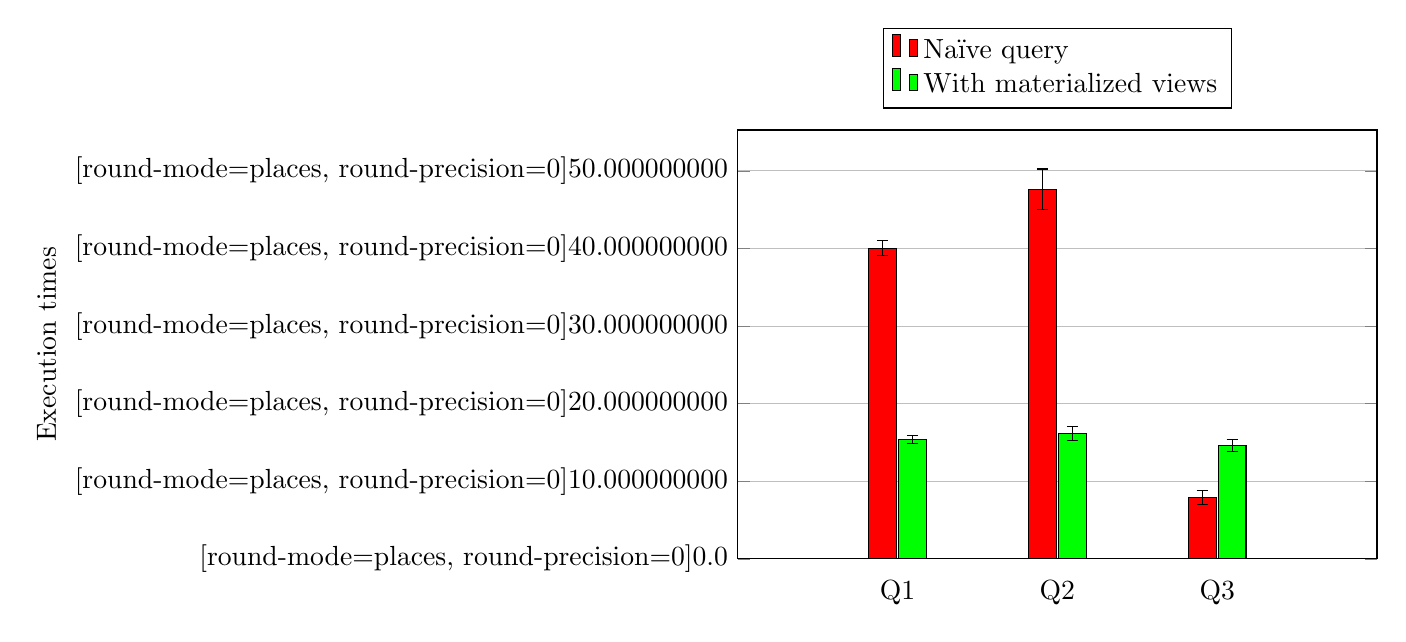
\begin{tikzpicture}
      \begin{axis}[
      width=.8\textwidth,
      height=20em,
      major x tick style = transparent,
      ybar=2*\pgflinewidth,
      %bar width=25pt,
      ylabel={Execution times},
      ymajorgrids = true,
      symbolic x coords={Q1,Q2,Q3},
      xtick = data,
      scaled y ticks = false,
      yticklabel={\SI[round-mode=places, round-precision=0]{\tick}{\s}},
      enlarge x limits=.5,
      ymin=0,
      legend cell align=left,
      legend style={at={(0.5,1.05)},anchor=south},
  ]
      \addplot[style={fill=red},error bars/.cd, y dir=both, y explicit]
          coordinates {
          (Q1,40.029) += (0,.971) -= (0,.971) %% (query_name, avg_cost) += (0,std) -= (0,std)
          (Q2,47.626) += (0,2.626) -= (0,2.626)
          (Q3,7.893) += (0,.915) -= (0,.915)};

      \addplot[style={fill=green},error bars/.cd, y dir=both, y explicit]
           coordinates {
          (Q1,15.392) += (0,.483) -= (0,.483)
          (Q2,16.153) += (0,.910) -= (0,.910)
          (Q3,14.608) += (0,.732) -= (0,.732)};

%      \addplot[style={fill=pink},error bars/.cd, y dir=both, y explicit]
%           coordinates {
%          (Q1,853) += (0,18) -= (0,18)
%          (Q2,165) += (0,27) -= (0,27)
%          (Q3,57) += (0,10) -= (0,10)};

%      \addplot[style={fill=blue},error bars/.cd, y dir=both, y explicit]
%           coordinates {
%           (Q1,4.33) += (0,0.2) -= (0,0.1)
%           (Q2,3.82) += (0,0.5) -= (0,0.2)
%           (Q3,3.82) += (0,0.5) -= (0,0.2)};

      \legend{Na\"{i}ve query, With materialized views, With indexes, With materialized views and indexes}
  \end{axis}
  \end{tikzpicture}
  \caption{Query timings}
  \label{fig:graph}
\end{figure}